\chapter{基于主动感知的多智能体交通资产检测方法与实验}
\label{chap:method_detection}

\section{引言}

尽管现有目标检测方法在通用视觉任务中已经取得了较高性能，但在交通资产清查场景下仍存在一定局限。具体而言，传统单次全图检测范式往往需要在固定输入分辨率与有限计算预算下同时处理小目标、边缘目标和密集目标，这使得模型在复杂背景、尺度压缩和局部遮挡条件下容易产生漏检；另一方面，即使采用更强的检测器，也通常只是提升单次前向推理的识别能力，难以对“哪些区域值得进一步复查”进行主动决策。因此，仅依赖单一检测器的静态推理流程，仍难以充分满足交通资产清查任务对目标发现完整性的要求。

针对上述问题，本文不再将交通资产检测视为一次性的静态推理任务，而是提出基于主动感知的多智能体改进思路：先在全图范围内完成初步检测，再根据场景内容与初检结果筛选值得重点复查的候选区域，随后开展局部精检并对多阶段结果进行融合。该思路通过将“目标检测”与“候选区域决策”解耦，旨在在有限计算预算下提升交通资产发现完整性。下文将围绕三阶段检测框架、Crop Agent 训练数据构建方法以及实验验证结果展开具体说明。


\section{基于异构 Agent 协作的三阶段检测框架}
\label{sec:three_stage_framework}

\subsection{总体框架概述}

设输入道路场景图像为 $I$，目标是输出图像中全部交通资产的类别标签与边界框集合。与传统检测器直接建立从 $I$ 到检测结果的单步映射不同，本文将检测过程拆分为“全局初检—候选区域推荐—局部精检—结果融合”三个阶段，并引入 Detection Agent 与 Crop Agent 的协同机制，将原本静态的一次性识别过程重构为面向潜在遗漏区域的主动感知流程。

图\ref{fig:framework_overview}给出了本文所提三阶段检测框架的整体结构。其中，Detection Agent 负责完成场景级检测与局部补检，Crop Agent 负责结合原始图像和初检结果生成具有高补检价值的候选区域，二者通过阶段化协作形成完整闭环。整体上，本文方法并不是简单地在原有检测流程后附加一次额外检测，而是通过“先发现、再判断、后复查”的方式，将有限计算资源优先分配到更可能存在遗漏目标的局部区域。

\begin{figure}[htbp]
    \centering
    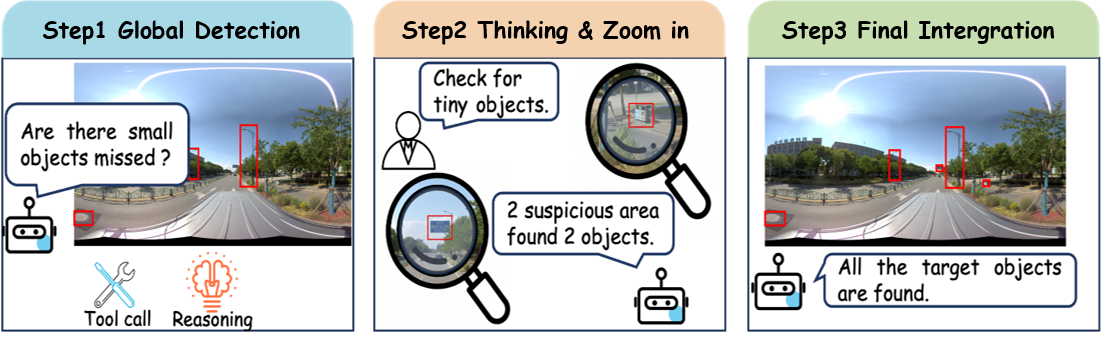
\includegraphics[width=\textwidth]{logo/三阶段检测框架图.png}
    \caption{基于主动感知的多智能体交通资产检测框架总体示意图}
    \label{fig:framework_overview}
\end{figure}

最终，系统对第一阶段与第三阶段结果进行融合，得到检测输出：
\begin{equation}
\mathcal{B}^{*} = \mathcal{F}\left(\mathcal{B}^{(1)}, \mathcal{B}^{(3)}\right),
\label{eq:final_fusion_general}
\end{equation}
其中，$\mathcal{B}^{(1)}$ 表示第一阶段全局初检结果，$\mathcal{B}^{(3)}$ 表示第三阶段局部精检结果，$\mathcal{F}(\cdot)$ 表示后处理融合函数。下面按照三阶段流程，分别介绍各阶段的功能定位与实现逻辑。

\subsection{第一阶段全局初检}

第一阶段中，Detection Agent 在整幅图像上执行全局检测，得到初始检测结果集合：
\begin{equation}
\mathcal{B}^{(1)} = f_{\mathrm{det}}^{(1)}(I),
\label{eq:stage1_detection}
\end{equation}
其中，$f_{\mathrm{det}}^{(1)}(\cdot)$ 表示第一阶段检测模型。

该阶段的主要任务是从场景整体尺度出发，对图像中的显著目标和易检目标进行快速扫描，建立初始的目标分布先验。它一方面为系统提供基础检测结果，另一方面也为第二阶段候选区域推荐提供关键信息输入。需要指出的是，第一阶段并不追求一次性穷尽全部目标，而是重点完成对场景内容的全局感知，为后续的重点复查提供依据。

\subsection{第二阶段候选区域推荐}

第二阶段中，Crop Agent 根据原始图像与第一阶段检测结果，生成候选裁剪区域集合：
\begin{equation}
\mathcal{C} = f_{\mathrm{crop}}(I, \mathcal{B}^{(1)}),
\label{eq:stage2_crop}
\end{equation}
其中，$\mathcal{C}=\{c_1,c_2,\dots,c_N\}$ 表示候选裁剪区域集合，$f_{\mathrm{crop}}(\cdot)$ 表示 Crop Agent。

与 Detection Agent 直接输出目标框不同，Crop Agent 的职责是决定“哪些区域值得再看”。它综合利用原始图像中的视觉上下文以及第一阶段提供的检测先验，对潜在的高价值区域进行筛选。这些区域通常对应于小目标聚集区域、密集目标区域、图像边缘区域或可能存在漏检的复杂背景区域。由此，第二阶段本质上承担的是一种面向补检的注意力重分配功能，即在有限推理预算下，将第三阶段的计算集中投放到最可能带来增量收益的位置。

\subsection{第三阶段局部精检与结果融合}

第三阶段中，Detection Agent 在每个裁剪区域上执行局部检测，得到局部补检结果：
\begin{equation}
\mathcal{B}^{(3)} = \bigcup_{c_i \in \mathcal{C}} f_{\mathrm{det}}^{(3)}(I_{c_i}),
\label{eq:stage3_detection}
\end{equation}
其中，$I_{c_i}$ 表示由候选区域 $c_i$ 从原图中裁剪得到的局部图像，$f_{\mathrm{det}}^{(3)}(\cdot)$ 表示第三阶段检测模型。

在这一阶段中，系统并不是简单地“再检测一次”，而是在第二阶段候选区域筛选的基础上，对高价值局部区域实施有针对性的精细感知。与第一阶段面向整图的全局初检不同，第三阶段的输入为经过尺度缩放的局部图像块。在这种观测条件下，目标的有效像素占比显著提升，背景噪声得到有效抑制。具体而言，局部精检具有三方面优势：首先，目标成像尺度的放大使边缘特征与内部纹理更易被检测器捕获；其次，局部视野降低了非相关背景对分类器的干扰，从而提升了信噪比；最后，在密集目标区域，局部推理能有效缓解大尺度特征图上的特征混叠，增强目标间的判别性。

如图 \ref{fig:local_refinement} 所示，通过对比全局初检与局部精检的预测分布可以发现，第三阶段能够显著恢复第一阶段中因尺度极小或排列过于密集而导致的遗漏目标。因此，第三阶段的作用应理解为对候选高价值区域的增量补检，而非对第一阶段结果的机械重复。

\begin{figure}[htbp]
    \centering
    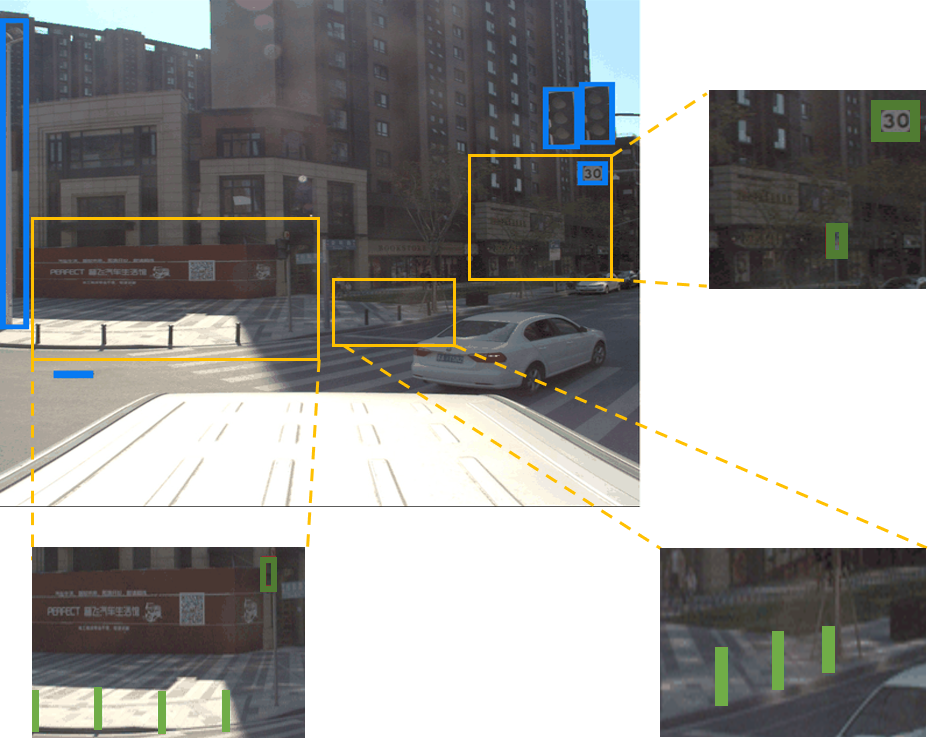
\includegraphics[width=\textwidth]{logo/第三阶段局部精检对遗漏目标的恢复示意图.png}
    \caption{第三阶段局部精检对遗漏目标的恢复示意图}
    \label{fig:local_refinement}
\end{figure}

由于第一阶段与第三阶段均独立输出边界框集合，系统还需进一步完成跨阶段结果融合。本文采用面向增量补检的轻量化融合策略：针对第三阶段输出的候选框，通过空间重叠度分析识别其增量价值。融合逻辑如图 \ref{fig:fusion_strategy} 所示，系统通过计算第三阶段预测框 $b$ 与第一阶段结果集 $\mathcal{B}^{(1)}$ 之间的交并比（IoU），识别并剔除冗余检测。本文设定的融合阈值为
\begin{equation}
\tau_f = 0.1.
\label{eq:fusion_threshold}
\end{equation}

因此，经过过滤后的第三阶段检测结果集合可表示为
\begin{equation}
\mathcal{B}^{(3)\prime}
=
\left\{
 b \in \mathcal{B}^{(3)}
 \;\middle|\;
 \max_{b' \in \mathcal{B}^{(1)}} \mathrm{IoU}(b,b') \le \tau_f
\right\},
\label{eq:filtered_stage3}
\end{equation}
最终融合结果为
\begin{equation}
\mathcal{B}^{*} = \mathcal{B}^{(1)} \cup \mathcal{B}^{(3)\prime}.
\label{eq:final_fusion}
\end{equation}

上述融合规则的核心思想在于：第三阶段主要负责补充第一阶段的遗漏结果，而不是重复覆盖第一阶段已检测到的目标。通过对第三阶段结果进行低阈值去重，可以有效抑制局部检测因尺度变化而带来的重复框问题，同时尽可能保留真正的新增补检结果。由此，最终输出结果可以自然地解释为“全局初检结果 + 局部补检结果”的增量融合。

\begin{figure}[htbp]
    \centering
    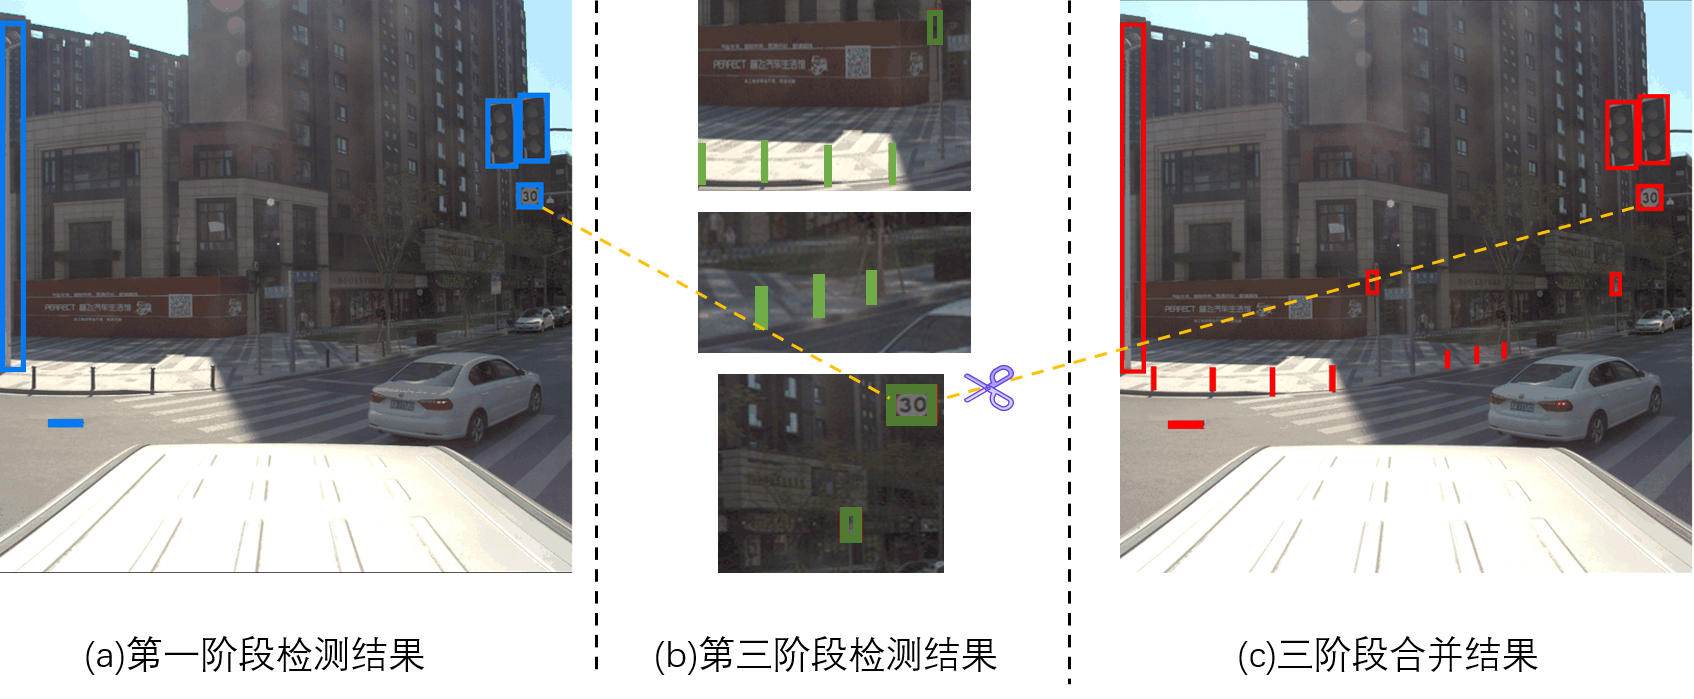
\includegraphics[width=\textwidth]{logo/第一阶段与第三阶段检测结果的融合示意图.png}
    \caption{第一阶段与第三阶段检测结果的融合示意图}
    \label{fig:fusion_strategy}
\end{figure}

\section{异构 Agent 协作机制与架构泛化性}

从协作关系上看，Detection Agent 与 Crop Agent 在本文框架中具有清晰的功能边界。Detection Agent 负责“识别并定位目标”，分别承担第一阶段的全局初检与第三阶段的局部精检；Crop Agent 负责“判断哪里值得再次观察”，根据原始图像和初检结果生成候选复查区域。通过这种职责划分，系统不再依赖单一模型在单次推理中同时完成全局扫描、区域决策与局部补检，而是将检测与候选区域推荐解耦为两个相互配合的功能模块。

这种解耦设计进一步带来了 Detection Agent 的架构泛化性。由于 Crop Agent 的功能定位是生成候选感兴趣区域（RoIs），而 Detection Agent 专注于特定尺度下的目标定位与分类，二者在任务逻辑上具备较强独立性。因此，任何具备“图像输入—边界框输出”能力的感知模型，均可作为 Detection Agent 接入本框架。基于此特性，第一阶段与第三阶段所使用的 Detection Agent 既可沿用基于视觉语言大模型（VLM）的检测器，也可灵活替换为 DINO、Faster R-CNN、DEIM、Grounding DINO 或 YOLO26 等主流检测器。

与之相对，第二阶段的 Crop Agent 在本研究中保持固定，其必要性主要体现在两个方面：一是模态兼容性，即 Crop Agent 需要协同处理“原始视觉信号”与“初检先验分布”的多模态输入，这要求基座模型具备较强的跨模态对齐能力；二是决策功能特化，即现有检测器主要针对目标回归任务设计，缺乏主动推理潜在遗漏区域的候选推荐机制。

在架构原型构建阶段，本文采用视觉语言大模型（VLM）RexOmni 作为 Detection Agent 与 Crop Agent 的统一基座。这样做的原因在于，Crop Agent 需要同时接收原始图像与第一阶段检测结果，RexOmni 所具备的跨模态表征能力更有利于将检测先验与视觉语义统一到同一隐空间中，从而支持候选区域推荐任务。为进一步验证该主动感知框架的通用性与鲁棒性，本文采用“固定感知策略，横向迁移检测器”的实验方案：在保持 Crop Agent 决策权重冻结的前提下，对 Detection Agent 进行模块化替换，系统性评估该框架在 DINO、Faster R-CNN、DEIM、Grounding DINO 及 YOLO26 等不同范式检测器上的适配表现。

综上所述，本文框架实质上构建了一种面向异构检测器的通用感知增强范式。它并非受限于特定模型的专用策略，而是通过引入主动感知闭环，系统性地提升了各类检测架构在复杂交通场景下的漏检抑制能力。
\begin{figure}[htbp]
    \centering
    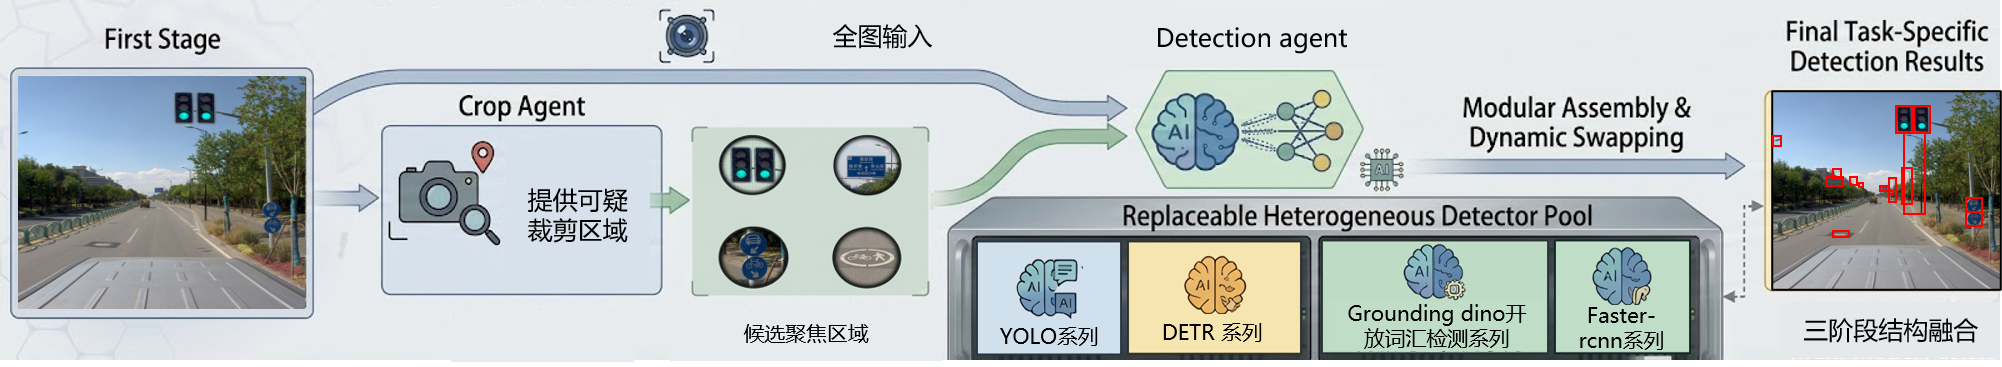
\includegraphics[width=\textwidth]{logo/裁剪 Agent 与异构 Detection Agent 的协作关系示意图.png}
    \caption{裁剪 Agent 与异构 Detection Agent 的协作关系示意图}
    \label{fig:heterogeneous_agents}
\end{figure}

\section{Crop Agent 的数据构造与训练}
\label{sec:crop_agent_data}

\subsection{小目标边界尺寸确定}

为了使 Crop Agent 的监督构造直接服务于小目标漏检补偿，本文首先需要对“小目标”给出与具体任务相一致的定量定义。与直接沿用通用目标检测数据集中的经验阈值不同，本文采用任务相关的性能统计结果来确定小目标边界尺寸。具体做法是：先在训练集上获得收敛的基础检测模型，再根据其在跨域测试集上的分尺度检测表现确定小目标边界阈值 $\tau_s$。有关阈值选取的统计依据与性能变化曲线将在本章实验部分给出。

在此基础上，本文将小目标集合与非小目标集合定义为：
\begin{equation}
\mathcal{B}_{\mathrm{small}}=\{b_i \mid s(b_i)<\tau_s\}, \qquad
\mathcal{B}_{\mathrm{large}}=\{b_i \mid s(b_i)\ge \tau_s\},
\label{eq:small_large_definition}
\end{equation}
其中，$s(b_i)$ 表示目标框 $b_i$ 的尺度表征函数。采用上述方式确定阈值的优势在于：其一，能够避免经验性阈值与当前任务场景不匹配的问题；其二，能够使小目标定义直接对应模型性能显著退化的关键区间，从而使 Crop Agent 的训练目标更加贴合交通资产检测中的真实漏检难点。

\subsection{第一阶段输入的监督构造}

Crop Agent 的输入需要同时包含“原始图像内容”和“第一阶段检测结果”。然而，在训练早期若直接使用不稳定的模型预测结果作为第一阶段输入，容易将噪声传播到裁剪区域学习过程中。为此，本文采用一种更稳定的监督构造方式：将武汉数据集中所有尺寸大于 $\tau_s$ 的真实目标框，作为“第一阶段检测结果”的替代输入，与原始图像共同送入 Crop Agent。

该设计具有三点作用。第一，大目标通常更容易被第一阶段检测器发现，用其模拟初检结果更符合实际推理场景；第二，通过人为屏蔽小目标，可促使 Crop Agent 学习“如何根据已发现目标与场景上下文去补找潜在遗漏区域”；第三，使用真实标注替代噪声检测结果，有助于提升 Crop Agent 训练过程的稳定性。因此，Crop Agent 的训练输入并不是“全量目标标注”，而是“原图 + 可视作第一阶段已发现结果的大目标集合”。

\subsection{基于区域生长的裁剪标注生成}

在确定小目标集合 $\mathcal{B}_{\mathrm{small}}$ 后，本文采用基于区域生长思想的方法构建 Crop Agent 的裁剪监督标签。其具体过程如下。
\begin{enumerate}
    \item 对每一个小目标真实框 $b_i \in \mathcal{B}_{\mathrm{small}}$，以其中心为基准，将宽和高同时向外扩展为原来的 $2$ 倍，得到外扩框 $\tilde{b}_i$；
    \item 若任意两个外扩框 $\tilde{b}_i$ 与 $\tilde{b}_j$ 存在相交，则认为它们属于同一候选生长区域；
    \item 对所有通过相交关系连通的外扩框进行合并，并取其最小外接矩形作为最终裁剪标注区域；
    \item 将得到的所有合并区域统一标注为类别 \texttt{crop\_region}。
\end{enumerate}

为便于形式化表达，记外扩框集合为 $\tilde{\mathcal{B}}=\{\tilde{b}_i\}$。若 $\tilde{b}_i \cap \tilde{b}_j \neq \varnothing$，则在图结构 $G=(V,E)$ 中连接一条边。对图 $G$ 的每一个连通分量 $\mathcal{C}_m$，定义其对应的裁剪监督区域为
\begin{equation}
r_m = \operatorname{MBR}\left( \bigcup_{\tilde{b}_i \in \mathcal{C}_m} \tilde{b}_i \right),
\label{eq:crop_region_gt}
\end{equation}
其中，$\operatorname{MBR}(\cdot)$ 表示最小外接矩形。最终，所有 $r_m$ 构成 Crop Agent 的监督标注集合。

上述构造方式具有两方面优势。其一，相比直接以单个小目标作为裁剪标注，合并后的区域更符合实际推理中“一个裁剪区域内包含多个潜在遗漏目标”的需求；其二，外扩操作为 Crop Agent 保留了必要的上下文信息，使第三阶段局部精检不仅关注目标本体，也能利用其周边纹理和结构线索。

\subsection{Crop Agent 的训练样本形式}

基于上述构造策略，本文将 Crop Agent 的单个训练样本组织为“图像 + 第一阶段输入结果 + 裁剪区域输出”三元组。输入端由原始图像及其对应的大目标集合构成，输出端为若干个类别为 \texttt{crop\_region} 的矩形框。由于 Crop Agent 的学习目标是区域推荐而非资产类别识别，因此其标签空间被约束为单一的区域类，从而将模型能力集中到“发现哪些地方值得复查”这一任务上。

\subsection{Crop Agent 的初始化方式}

考虑到 Crop Agent 的任务与 Detection Agent 在表征层面存在较强关联，本文并未直接从随机状态或无关模型出发训练 Crop Agent，而是以 RexOmni 为基础继续训练。此外，本文还在实验中进一步比较两种初始化方式：其一，直接基于预训练后的 RexOmni 训练 Crop Agent；其二，基于已经在武汉数据集上微调收敛的 RexOmni 再训练 Crop Agent。该对比用于分析领域适配初始化是否能够进一步提升候选区域推荐质量，相关实验结果将在本章实验部分给出。

\section{实验验证与结果分析}
\label{sec:exp_setup}

\subsection{实验目标}

本章后续实验围绕前文提出的“全局初检—候选区域推荐—局部精检—结果融合”三阶段框架展开验证，重点回答以下五个问题：
\begin{enumerate}
    \item 所提出的三阶段主动感知检测框架，是否能够在交通资产检测任务上相较于原始检测器取得稳定性能增益；
    \item 该框架对于小目标、密集目标以及复杂背景区域中的目标检测，是否具有更明显的改进效果；
    \item 该框架是否具有检测器无关性，即能否在不同类型的 Detection Agent 上均表现出一致有效性；
    \item 在训练 Crop Agent 时，基于预训练 RexOmni 初始化与基于武汉数据集微调收敛后的 RexOmni 初始化，二者是否会对最终性能产生差异；
    \item 框架中的关键组成部分，尤其是候选区域推荐与局部精检机制，分别对最终性能起到了怎样的作用。
\end{enumerate}

为回答上述问题，本文从实验数据与评价设置、整体性能与跨检测器对比、小目标与密集目标分析、消融实验以及方法局限性分析五个层面展开实验。

\subsection{数据集与评估指标}

本章实验所使用的数据集基于第二章所述的 WHU-Infra3D 道路基础设施数据集开展\cite{whu_infra3d_2025}。该数据集由移动测绘系统采集，包含高分辨率全景图像、激光雷达点云及多层次标注信息。考虑到本文研究目标聚焦于二维视觉检测任务，实验中仅使用其中的图像数据及对应的二维边界框标注，而不引入点云语义标签、实例分割或属性状态等三维信息。需要进一步说明的是，本文在第三章实验中实际使用的输入图像并非原始 ERP 全景图，而是由每张全景图经过四分投影切割后得到的 $4$ 张透视结果图像。

在具体实验协议上，本文采用“武汉训练、上海测试”的跨城市设置。训练阶段使用武汉子集完成 Detection Agent 的场景适配以及 Crop Agent 的数据构建与训练，实验共构建出 6712 张四分投影后的透视训练图像，并选取其中 50\% 构建对应的 Crop Agent 训练数据。测试阶段使用上海子集的 4700 张四分投影透视图像评估模型在域偏移条件下的泛化能力。数据集共提供面向 10 类道路基础设施的二维标注，涵盖交通标志、路灯、信号灯、监控摄像头、路桩、消防栓、垃圾桶、井盖等典型城市设施。由于上海与武汉在采集时间、道路环境、目标密度、遮挡状况及光照变化等方面存在明显差异，该实验设置能够较好反映真实应用中模型跨城市迁移时面临的域偏移问题\cite{whu_infra3d_2025}。

为更细致地反映模型在不同尺度目标上的检测能力，本文采用分尺度评估策略。具体而言，本文首先统计基础检测模型在不同目标尺寸区间上的 F1-score 变化曲线，如图~\ref{fig:small_object_threshold} 所示。可以看出，当目标尺寸减小至 50 像素附近后，F1-score 出现明显下降，说明该尺度以下目标已成为检测器的主要感知困难区域。据此，本文将小目标边界尺寸确定为 $\tau_s=50$。在后续实验中，当目标长宽均大于该阈值时，将其视为大目标；否则视为小目标。

\begin{figure}[htbp]
    \centering
    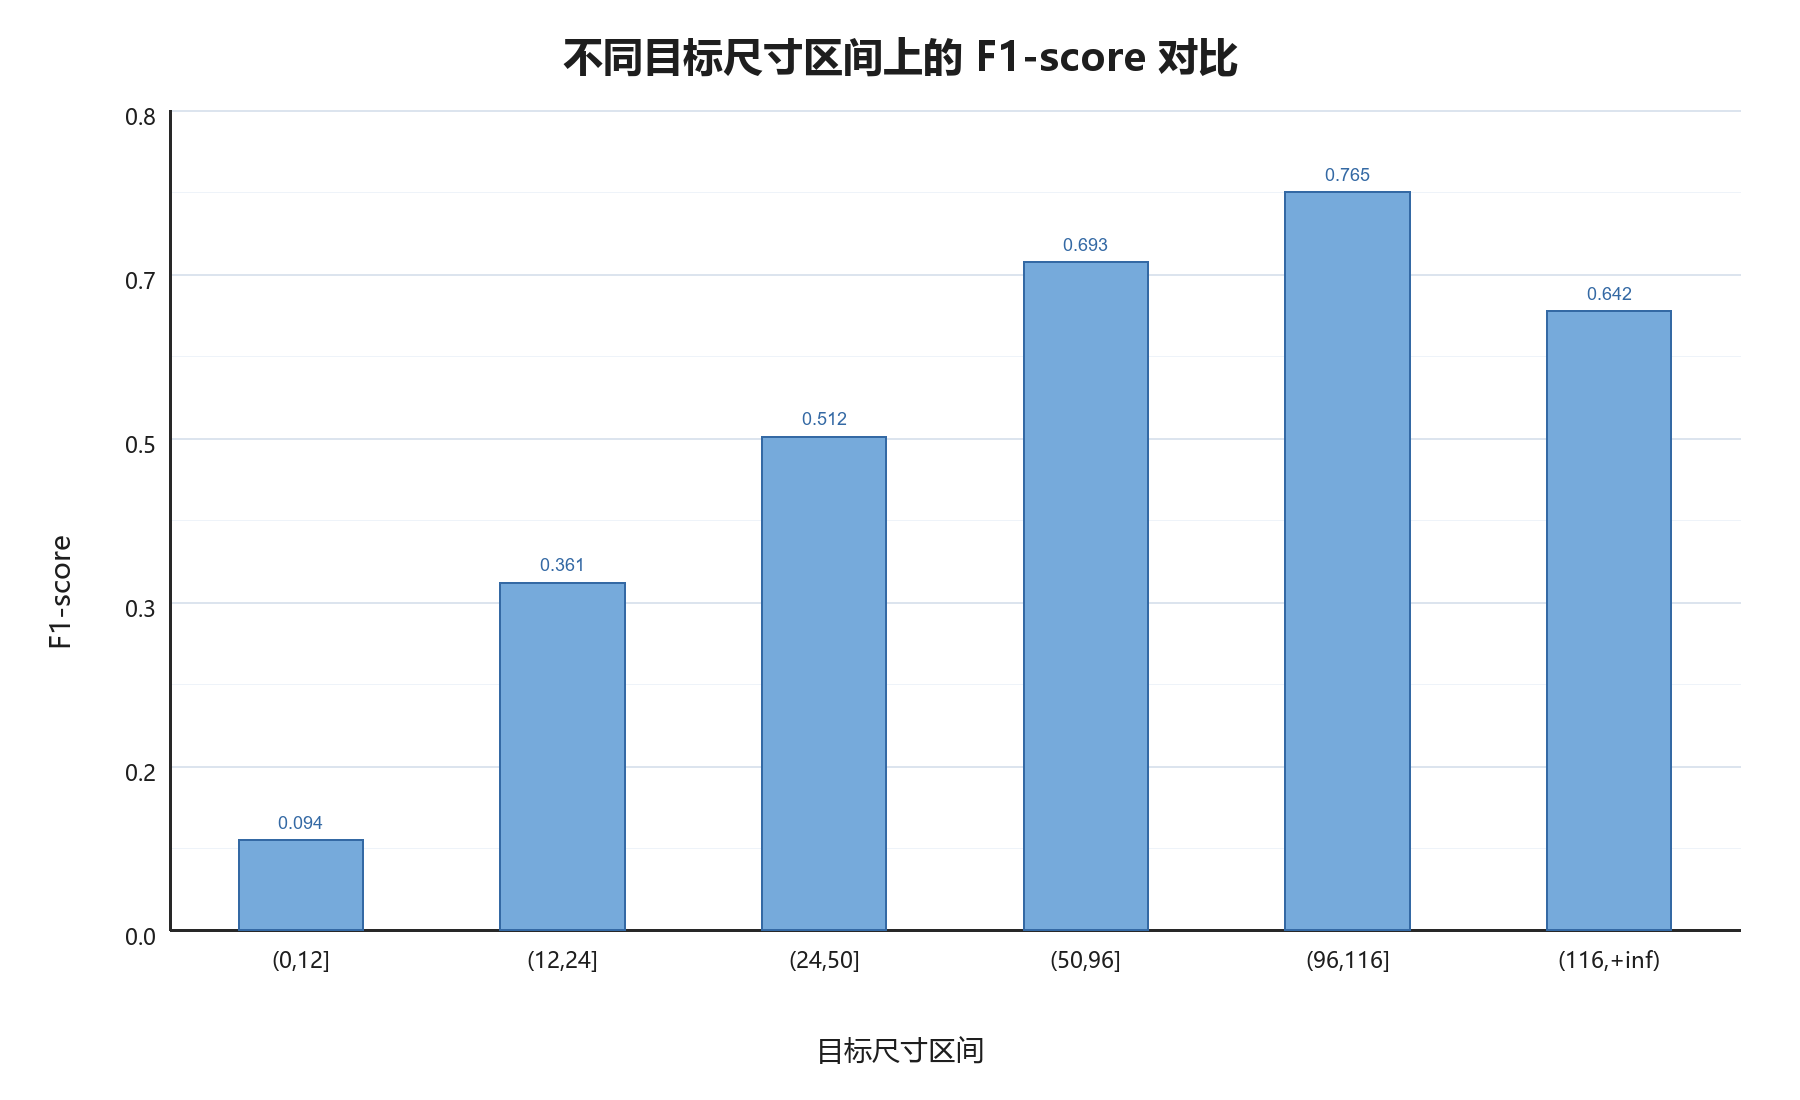
\includegraphics[width=0.75\textwidth]{logo/小目标阈值确定曲线.png}
    \caption{不同目标尺寸区间上的 F1-score 变化曲线及小目标阈值确定结果}
    \label{fig:small_object_threshold}
\end{figure}

评价时采用差异化 IoU 匹配阈值：大目标使用 IoU$=0.5$，小目标使用 IoU$=0.1$。该设置与本文任务中小目标占比较高、且边界框轻微偏移即可导致常规 IoU 严重下降的特点相一致。

在评价指标方面，本文主要采用 Precision、Recall、F1-score、mIoU、Macro-F1、Micro-F1 以及 Micro-IoU综合评价。其定义如下：
\begin{equation}
\mathrm{Precision}=\frac{TP}{TP+FP},
\qquad
\mathrm{Recall}=\frac{TP}{TP+FN},
\label{eq:precision_recall_exp}
\end{equation}
\begin{equation}
F1=\frac{2\cdot \mathrm{Precision}\cdot \mathrm{Recall}}
{\mathrm{Precision}+\mathrm{Recall}},
\label{eq:f1_exp}
\end{equation}
\begin{equation}
\mathrm{IoU}_c=\frac{TP_c}{TP_c+FP_c+FN_c},
\label{eq:iou_exp}
\end{equation}
\begin{equation}
mIoU=\frac{1}{K}\sum_{c=1}^{K}\mathrm{IoU}_c,
\label{eq:miou_exp}
\end{equation}
其中，$TP$、$FP$ 和 $FN$ 分别表示真阳性、假阳性和假阴性数量，$K$ 表示类别总数。

为明确区分 Macro 与 Micro 统计口径，本文进一步定义：
\begin{equation}
F1_c=\frac{2P_cR_c}{P_c+R_c},\qquad
\mathrm{Macro\text{-}F1}=\frac{1}{K}\sum_{c=1}^{K}F1_c,
\label{eq:macro_f1_exp}
\end{equation}
\begin{equation}
\mathrm{Micro\text{-}F1}
=\frac{2\sum_{c=1}^{K}TP_c}
{2\sum_{c=1}^{K}TP_c+\sum_{c=1}^{K}FP_c+\sum_{c=1}^{K}FN_c},
\label{eq:micro_f1_exp}
\end{equation}
\begin{equation}
\mathrm{Micro\text{-}IoU}
=\frac{\sum_{c=1}^{K}TP_c}
{\sum_{c=1}^{K}TP_c+\sum_{c=1}^{K}FP_c+\sum_{c=1}^{K}FN_c}.
\label{eq:micro_iou_exp}
\end{equation}

其中，Macro-F1 对每个类别赋予相同权重，更能反映长尾类别与小样本类别的整体表现；Micro-F1 对所有样本统一汇总，更偏向反映高频类别上的总体识别效果。类似地，mIoU 是“先按类别计算 IoU 再平均”，强调各类别均衡性；Micro-IoU 是“全类别 TP/FP/FN 汇总后计算 IoU”，更强调全局检测质量与主流类别贡献。

\subsection{对比方法}

为了验证所提出框架的泛化能力，本文选取了六种类型差异较大的检测器作为 Detection Agent：RexOmni、DINO、Faster R-CNN、DEIM、Grounding DINO 和 YOLO26 。对所有模型，均分别评估其原始检测结果，以及接入本文“全局初检—候选区域推荐—局部精检—结果融合”三阶段流程后的增强结果。实验执行顺序严格遵循两阶段协议：先完成“RexOmni Detection Agent + RexOmni Crop Agent”的同源训练与验证，再扩展到“固定 Crop Agent、替换 Detection Agent”的异构检测器对比。

需要强调的是，本文方法不改动基础检测器的检测头结构。实验核心不是比较不同 backbone 或 neck，而是比较“\textbf{原始检测器}”与“\textbf{原始检测器 + 三阶段主动感知框架}”之间的差异。

此外，本文的 Crop Agent 并非从零训练，而是由已完成基础检测适配的 RexOmni 继续训练得到。其原因是：已有检测 Agent 已具备“物体大致位置感知”能力，继续训练时只需将优化目标切换为高价值候选区域推荐。为保证可比性，本章异构对比实验中 Crop Agent 保持固定，仅替换第一、三阶段的 Detection Agent。

\begin{table}[htbp]
    \centering
    \caption{实验中采用的对比检测器}
    \label{tab:compared_detectors}
    \begin{tabular}{llll}
        \toprule
        检测器 & 类型 & 在框架中的角色 & 实验配置 \\
        \midrule
        RexOmni & 大模型检测器 & Detection Agent & 原始 / 接入三阶段框架 \\
        DINO & Transformer 检测器 & Detection Agent & 原始 / 接入三阶段框架 \\
        Faster R-CNN & 两阶段检测器 & Detection Agent & 原始 / 接入三阶段框架 \\
        DEIM & 通用目标检测器 & Detection Agent & 原始 / 接入三阶段框架 \\
        Grounding DINO & 开放词汇检测器 & Detection Agent & 原始 / 接入三阶段框架 \\
        YOLO26 & 单阶段检测器 & Detection Agent & 原始 / 接入三阶段框架 \\
        \bottomrule
    \end{tabular}
\end{table}

\subsection{实现细节}

在实验过程中，本文统一遵循本章前文提出的三阶段检测流程。第一阶段在整幅图像上执行全局初检，得到初始检测框集合；第二阶段由 Crop Agent 根据原图与初检结果生成候选裁剪区域；第三阶段在候选区域内执行局部精检；最终通过结果融合策略获得最终检测输出。

需要说明的是，所有基于 RexOmni 的训练均采用与 RexOmni 原论文一致的奖励函数与训练设置 \cite{rexomni2025}。本文在方法章节中不展开其具体奖励项设计，而在实验部分仅说明：不论是 Detection Agent 的同源训练，还是 Crop Agent 的继续训练，均保持与原始 RexOmni 一致的奖励范式，以保证训练目标和结果具有可比性。

为保证不同检测器之间的实验具有可比性，本文在所有对比模型上尽可能保持一致的候选区域生成逻辑以及融合策略。特别地，在结果融合阶段，首先将第三阶段局部检测结果映射回原图坐标系，再与第一阶段检测结果进行重复框筛除；当第三阶段检测框与第一阶段任一检测框的 IoU 小于固定阈值 $\tau_f=0.1$ 时，该框才作为新增补检结果保留，否则视为重复检测并删除，从而避免重复框对最终统计结果造成干扰。

\subsection{整体性能对比}
\label{sec:overall_comparison}

\subsubsection{总体结果与跨检测器泛化分析}

表~\ref{tab:overall_main_results} 给出了不同检测器在原始检测设置与接入本文框架后的整体性能对比结果。总体来看，三阶段主动感知流程在多种类型 Detection Agent 上均能够带来稳定性能提升，说明该方法并非仅对特定检测器有效，而具有较好的检测器无关性与泛化能力。

从六个检测器的结果看，Macro-F1、Micro-F1、mIoU 和 Micro-IoU 均呈现提升趋势，平均绝对增益分别为 +8.18\%、+6.41\%、+2.90\% 和 +2.53\%。这一结果具有两层含义：其一，Macro-F1 增益高于 Micro-F1，说明改进并非只来自高频类别，而是对长尾类别也有实质补益；其二，mIoU 与 Micro-IoU 同步上升，表明提升不仅体现在“检出来更多”，也体现在“框匹配更合理”。

从结果性质上看，这种提升并不意味着框架仅通过增加预测框数量获得收益，而是说明通过“候选区域推荐 + 局部精检”机制，模型能够在原始全图检测基础上有效恢复部分遗漏目标，尤其是在小尺度和复杂区域目标上提升 Recall，并在合理控制 Precision 波动的前提下推动整体 F1 提升。

进一步观察不同模型的收益幅度可以发现：Faster R-CNN、DEIM、DINO 和 YOLO26 的增幅更大；Grounding DINO 与 RexOmni 在较高基线上仍保持稳定提升。以 Grounding DINO 为例，其 Micro-F1 从 0.7665 提升至 0.7816，mIoU 从 0.4944 提升至 0.5154，说明即使在较强基线模型上，局部再检测与增量融合机制仍然有效。

结合“武汉训练—上海测试”的跨城设置，这些结果进一步说明：本文方法并非依赖单一模型结构，而是在明显域偏移下仍能稳定提升检测完整性与匹配质量，具有较好的跨场景泛化潜力。进一步从模型类型看，无论基础模型属于大模型检测器、单阶段检测器、两阶段检测器还是开放词汇检测器，接入本文框架后均获得正向收益。这说明本文框架所解决的并不是某一类检测器特有的偏差问题，而是交通资产检测中更普遍的“单次全图检测难以兼顾全局覆盖与局部精检”问题。由于 Crop Agent 在本章实验中保持固定，仍能稳定增强异构 Detection Agent，因此也说明由 RexOmni 继续训练得到的候选区域推荐策略具有较强的外部可迁移性。

\begin{table}[htbp]
    \centering
    \caption{不同检测器接入本文框架前后的整体性能对比}
    \label{tab:overall_main_results}
    \resizebox{0.95\textwidth}{!}{
    \begin{tabular}{lcccccccccccc}
        \toprule
        \multirow{2}{*}{检测器} & \multicolumn{3}{c}{Macro-F1} & \multicolumn{3}{c}{Micro-F1} & \multicolumn{3}{c}{mIoU} & \multicolumn{3}{c}{Micro-IoU} \\
        \cmidrule(lr){2-4} \cmidrule(lr){5-7} \cmidrule(lr){8-10} \cmidrule(lr){11-13}
        & 前 & 后 & $\Delta$(\%) & 前 & 后 & $\Delta$(\%) & 前 & 后 & $\Delta$(\%) & 前 & 后 & $\Delta$(\%) \\
        \midrule
        RexOmni & 0.6148 & 0.6328 & +1.80 & 0.6770 & 0.6853 & +0.83 & 0.3705 & 0.3828 & +1.23 & 0.4231 & 0.4264 & +0.33 \\
        DINO & 0.5308 & 0.5778 & +4.70 & 0.5878 & 0.6354 & +4.76 & 0.3163 & 0.3531 & +3.68 & 0.3668 & 0.4057 & +3.89 \\
        Faster R-CNN & 0.1322 & 0.3803 & +24.81 & 0.2515 & 0.4370 & +18.55 & --- & --- & --- & --- & --- & --- \\
        DEIM & 0.4265 & 0.5300 & +10.35 & 0.5108 & 0.5940 & +8.32 & 0.2322 & 0.3000 & +6.78 & 0.2934 & 0.3524 & +5.90 \\
        Grounding DINO & 0.7279 & 0.7486 & +2.07 & 0.7665 & 0.7816 & +1.51 & 0.4944 & 0.5154 & +2.10 & 0.5360 & 0.5525 & +1.65 \\
        YOLO26 & 0.4345 & 0.4879 & +5.34 & 0.5206 & 0.5654 & +4.48 & 0.2504 & 0.2863 & +3.59 & 0.3153 & 0.3493 & +3.40 \\
        \bottomrule
    \end{tabular}}
\end{table}

\subsubsection{大目标与整体结果的关系}

进一步观察分尺度统计结果可以发现，本文方法的主要收益并非来自大目标重复检测，而是来自小目标与疑难区域补检。六个检测器中，大目标 Micro-F1 平均增益仅为 +0.04\%，而小目标 Micro-F1 平均增益为 +9.30\%，显著更高。

这一现象与本文方法设计初衷一致：第一阶段建立全局检测基线，第二、三阶段将计算资源聚焦到“边缘疑难区、小物体聚集区、多目标密集区”。因此，本文框架可以被视为一种面向漏检恢复的增量式增强策略。

\begin{table}[htbp]
    \centering
    \caption{不同检测器在分尺度下的增益对比（单位：\%）}
    \label{tab:scale_results}
    \begin{tabular}{lcccc}
        \toprule
        检测器 & \shortstack{$\Delta$大目标\\Micro-F1} & \shortstack{$\Delta$小目标\\Micro-F1} & \shortstack{$\Delta$整体\\Micro-F1} & \shortstack{$\Delta$小目标\\Recall} \\
        \midrule
        RexOmni & -0.07 & +1.30 & +0.83 & +5.56 \\
        DINO & +0.07 & +6.66 & +4.76 & +9.05 \\
        Faster R-CNN & +0.31 & +27.39 & +18.55 & +25.17 \\
        DEIM & -0.04 & +11.97 & +8.32 & +14.80 \\
        Grounding DINO & -0.09 & +2.12 & +1.51 & +5.32 \\
        YOLO26 & +0.08 & +6.33 & +4.48 & +6.73 \\
        \bottomrule
    \end{tabular}
\end{table}

\subsection{小目标与密集目标检测性能分析}
\label{sec:small_dense_analysis}

\subsubsection{小目标检测性能提升分析}

交通资产检测场景中，大量目标具有尺寸小、纹理弱、与背景相似度高等特点，这使得小目标检测成为评价检测系统实用性的关键环节。本文提出的三阶段主动感知框架，正是针对这类目标在全图检测中容易被忽略的问题而设计。

从六个检测器的小目标结果看，提升主要体现为 Recall 增长并带动 F1 提升。以 DEIM 为例，小目标 Recall 从 0.3389 提升至 0.4869（+14.80\%），Micro-F1 从 0.4442 提升至 0.5639（+11.97\%）；YOLO26 的小目标 Recall 从 0.3344 提升至 0.4017（+6.73\%），Micro-F1 从 0.4528 提升至 0.5161（+6.33\%）；DINO 的小目标 Recall 从 0.4346 提升至 0.5251（+9.05\%），Micro-F1 从 0.5302 提升至 0.5968（+6.66\%）。该现象说明主动裁剪与局部精检能够有效恢复全图检测遗漏的小尺度目标。

值得注意的是，小目标提升并不是通过简单放宽阈值或堆叠预测框获得，而是通过候选区域推荐机制将检测资源重新分配到高价值局部区域。在局部裁剪后，小目标有效尺度被放大、背景干扰被压缩，因此不同检测器都能获得一致的小目标补检收益。

\begin{table}[htbp]
    \centering
    \caption{不同检测器在小目标上的性能对比}
    \label{tab:small_results}
    \resizebox{\textwidth}{!}{
    \begin{tabular}{lcccccc}
        \toprule
        检测器 & Recall（前） & Recall（后） & $\Delta$Recall（\%） & Micro-F1（前） & Micro-F1（后） & $\Delta$Micro-F1（\%） \\
        \midrule
        RexOmni & 0.5667 & 0.6223 & +5.56 & 0.6489 & 0.6619 & +1.30 \\
        DINO & 0.4346 & 0.5251 & +9.05 & 0.5302 & 0.5968 & +6.66 \\
        Faster R-CNN & 0.0860 & 0.3377 & +25.17 & 0.1368 & 0.4107 & +27.39 \\
        DEIM & 0.3389 & 0.4869 & +14.80 & 0.4442 & 0.5639 & +11.97 \\
        Grounding DINO & 0.6408 & 0.6940 & +5.32 & 0.7403 & 0.7615 & +2.12 \\
        YOLO26 & 0.3344 & 0.4017 & +6.73 & 0.4528 & 0.5161 & +6.33 \\
        \bottomrule
    \end{tabular}}
\end{table}

从表~\ref{tab:small_results} 可见，六个检测器的小目标 Recall 全部为正增益，进一步验证了本文方法的核心作用是“漏检恢复”。虽然部分模型的 Precision 会有轻微波动，但 Recall 的提升幅度更大，因此最终 F1 普遍上升。

\subsubsection{密集目标、复杂区域与典型案例分析}

除小目标外，密集目标区域同样是交通资产检测中的典型难点。此类区域往往包含多个相邻目标、结构相似目标或者排列紧凑目标，模型在全图尺度下容易出现相互遮蔽、重复抑制或部分遗漏等问题。

本文框架对这类区域的改进主要体现在两个方面。首先，Crop Agent 候选区域推荐机制能够主动识别高密度目标分布区域，并将这些区域作为第三阶段重点检测对象；其次，局部精检阶段能够在更小视野内重新解析目标间的边界关系，从而提升相邻目标之间的可分性。对于交通标志群、连续路灯、密集路桩以及复杂路侧设施区域，这种机制通常能够带来更好的目标分离效果。

从实验现象看，接入本文三阶段检测框架后的结果在复杂道路边缘区域、远距离设施聚集区域以及多目标并列区域中，能够恢复更多此前被遗漏的目标。这说明主动感知机制不仅提高了单个小目标的被发现概率，也改善了复杂区域的整体可解析性。结合可视化结果，本文方法的典型有效场景主要包括三类：其一，远距离小目标恢复场景，例如远处交通灯、细长路桩和小型监控设备在全图检测中常被忽略，而在局部裁剪后能够被成功识别；其二，密集目标分离场景，例如多个相邻交通标志、连续排列路灯或路侧设施聚集区域，局部精检有助于重新分离相邻目标边界，减少漏检与粘连；其三，图像边缘与局部复杂背景场景，在此类区域中目标仅占据局部视野的一部分且背景纹理干扰较强，通过候选区域推荐与局部检测，模型能够获得更聚焦的感知视野，从而提升检测稳定性。

\begin{figure}[htbp]
    \centering
    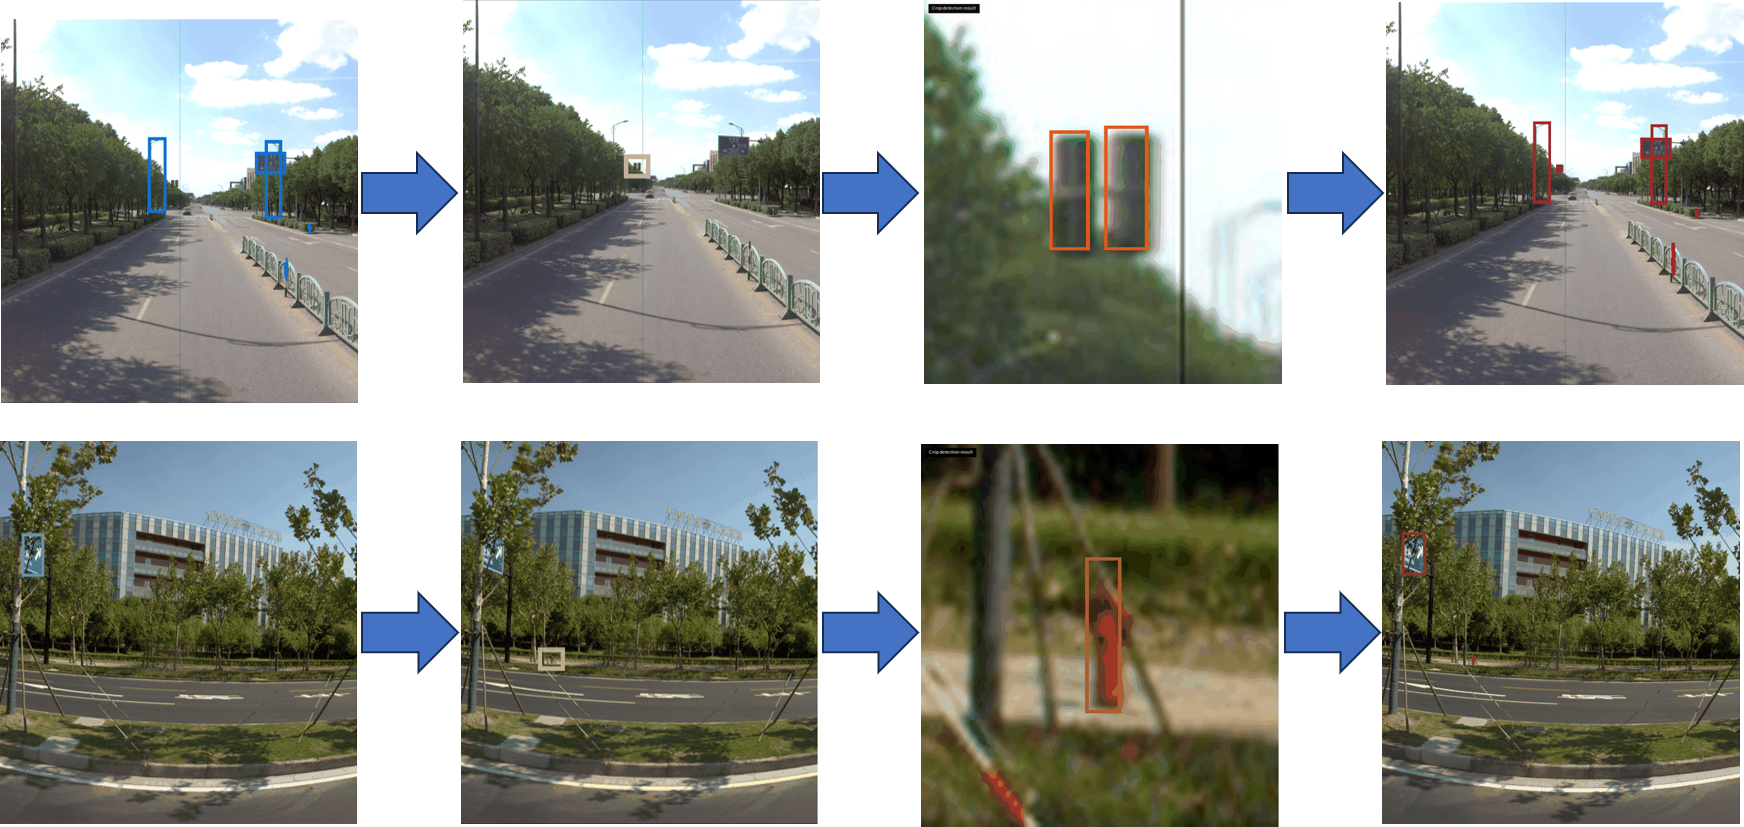
\includegraphics[width=\textwidth]{logo/小目标检测结果可视化对比.png}
    \caption{小目标检测结果可视化对比}
    \label{fig:small_object_cases}
\end{figure}

\begin{figure}[htbp]
    \centering
    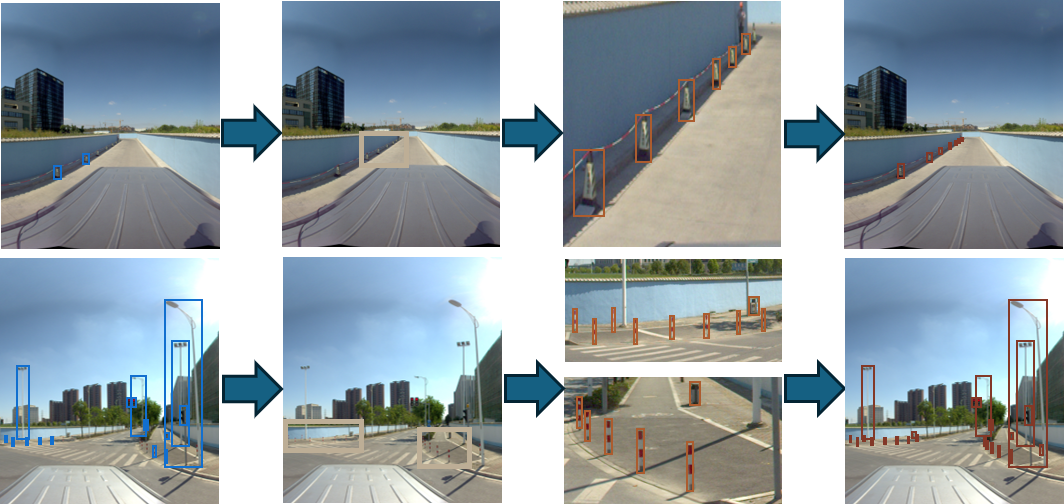
\includegraphics[width=\textwidth]{logo/密集区域检测结果可视化对比.png}
    \caption{密集区域检测结果可视化对比}
    \label{fig:dense_region_cases}
\end{figure}

\subsection{消融实验}
\label{sec:ablation_study}

\subsubsection{三阶段结构有效性分析}

为验证本文所提出三阶段主动感知检测流程的结构有效性，本节将“全图检测两次并融合”与“完整三阶段框架”进行对比。其中，前者表示在相同 Detection Agent 下，两次检测都直接作用于原始整图，并将两次全图检测结果进行统一融合；后者则采用第一阶段全图初检、第二阶段候选区域推荐、第三阶段局部精检以及最终结果融合的完整流程。

该对比的核心目的在于区分“检测次数增加”与“主动感知策略引入”这两种因素的作用。若仅将检测器在全图上重复执行一次，系统虽然增加了推理次数，但并未改变观测尺度与注意力分配方式；而完整三阶段框架则通过候选区域推荐与局部精检，将第二次观察聚焦到更可能存在遗漏目标的局部区域。
% 因此，若完整三阶段框架优于“全图检测两次并融合”，则说明本文方法的优势在于局部高价值区域的针对性再检测，而不是简单重复全图推理。

\begin{table}[htbp]
    \centering
    \caption{三阶段主动感知框架结构消融实验}
    \label{tab:ablation_framework}
    \begin{tabular}{lcccc}
        \toprule
        方法设置 & Macro-F1 & Micro-F1 & mIoU & Micro-IoU \\
        \midrule
        全图检测两次并融合 & -- & -- & -- & -- \\
        完整三阶段框架 & 0.6328 & 0.6853 & 0.3828 & 0.4264 \\
        \bottomrule
    \end{tabular}
\end{table}

\subsubsection{候选裁剪策略对比}

除三阶段整体结构外，本文还进一步比较 Crop Agent 引导裁剪与规则裁剪策略之间的差异，以分析性能增益究竟来自“局部分辨率提升”本身，还是来自“高价值区域的主动选择”。为此，本文设计如下两种对比方案：
\begin{enumerate}
    \item \textbf{固定步长重叠滑窗切片检测}：对输入的 $8192\times 4096$ 全景图像采用 $sub\_size=1024$、$stride=512$ 的重叠滑窗方式进行规则切片。按照该设置，图像在水平方向可生成 15 个窗口，在垂直方向可生成 7 个窗口，因此共得到 105 个局部子块。随后，对全部子块分别执行检测，并将检测结果映射回原图坐标系后统一融合。
    \item \textbf{主动感知三阶段检测}：先进行第一阶段全图初检，再由第二阶段 Crop Agent 根据原图内容与初检结果预测候选区域，最后在第三阶段对这些候选区域执行局部精检并与初检结果融合。
\end{enumerate}

需要说明的是，上述固定步长滑窗切片检测\textbf{未对全景图像进行透视投影}，而是直接在 ERP 图像上切片。这是因为本文采用的 $1024\times1024$ 局部窗口相对于 $8192\times4096$ 全景图仅对应约 $45^\circ\times45^\circ$ 的局部视场。在该尺度下，若切片位于道路场景常见的地平线附近，则 ERP 的局部尺度变化较小，其水平拉伸因子在 $\pm22.5^\circ$ 纬度范围内最大约为 $\sec 22.5^\circ \approx 1.08$，可近似视为缓慢变化的局部仿射形变。已有研究也指出，ERP 图像的显著畸变主要集中在靠近极区的位置，而地平线附近的局部畸变相对较弱\cite{yang2018equirectangular_detection,wang2022landmarks}。结合本文交通资产主要分布在道路两侧、整体接近地平线带的场景特征，可以认为此时切片内的几何畸变基本可忽略。

若进一步对全部滑窗子块执行透视重投影，则需要对 105 个候选窗口逐一完成球面到平面的变换，并额外处理坐标映射与结果融合，计算与实现开销均会明显增加。相关工作同样表明，多切平面投影虽然能够改善几何一致性，但通常伴随较高的计算代价\cite{zhang2018saliency360,su2019ktn}。因此，在该对照实验中继续对小切片做透视投影得不偿失。基于此，本文将固定滑窗策略设定为“直接在 ERP 图像上切片检测”，以作为主动感知裁剪的规则基线。

上述对比的核心在于：前者属于\textbf{穷举式规则裁剪}，其覆盖充分但计算冗余较高，且无法区分“值得复查的区域”与“低价值背景区域”；后者则属于\textbf{任务驱动的自适应裁剪}，其目标是在有限的局部检测预算下，优先将第二次观测分配给更可能存在漏检目标的区域。因此，该实验能够更直接地回答：主动感知机制的收益是否主要来源于 Crop Agent 对高价值候选区域的选择能力。

实验选取 DINO 与 YOLO26 作为代表性 Detection Agent，分别对应基于 Transformer 的检测器与实时单阶段检测器。这样的设置有助于观察：对于不同范式的基础检测器，主动感知裁剪与固定滑窗裁剪在检测收益和适配性上是否具有一致表现。

\begin{table}[htbp]
    \centering
    \caption{不同候选裁剪策略下的总体检测指标对比}
    \label{tab:ablation_crop_agent}
    \resizebox{\textwidth}{!}{
    \begin{tabular}{llcccccc}
        \toprule
        检测器 & 方法设置 & Precision & Recall & Macro-F1 & Micro-F1 & mIoU & Micro-IoU \\
        \midrule
        DINO & 固定步长重叠滑窗切片检测 & 0.5837 & 0.5373 & 0.4940 & 0.5596 & 0.3096 & 0.3647 \\
        DINO & 主动感知三阶段检测 & 0.7135 & 0.5727 & 0.5778 & 0.6354 & 0.3531 & 0.4057 \\
        YOLO26 & 固定步长重叠滑窗切片检测 & 0.6723 & 0.4885 & 0.5280 & 0.5658 & 0.3364 & 0.3786 \\
        YOLO26 & 主动感知三阶段检测 & 0.7369 & 0.4587 & 0.4879 & 0.5654 & 0.2863 & 0.3493 \\
        \bottomrule
    \end{tabular}}
\end{table}

从表~\ref{tab:ablation_crop_agent} 可以看出，主动感知三阶段检测相对于固定步长重叠滑窗切片检测的优势，主要体现在更高的候选区域利用效率与更优的精度--召回平衡。对于 DINO，主动感知方案在全部总体指标上均优于规则滑窗：Precision、Recall、Macro-F1、Micro-F1、mIoU 和 Micro-IoU 分别由 0.5837、0.5373、0.4940、0.5596、0.3096 和 0.3647 提升至 0.7135、0.5727、0.5778、0.6354、0.3531 和 0.4057。该结果表明，Crop Agent 带来的收益并非单纯来自局部分辨率提升，而是来源于更有效的候选区域筛选与更稳定的局部精检。

\begin{table}[htbp]
    \centering
    \caption{不同候选裁剪策略下的分尺度检测指标对比}
    \label{tab:ablation_crop_agent_scale}
    \resizebox{\textwidth}{!}{
    \begin{tabular}{lllcccc}
        \toprule
        检测器 & 目标尺度 & 方法设置 & Precision & Recall & Macro-F1 & Micro-F1 \\
        \midrule
        DINO & 大目标 & 固定步长重叠滑窗切片检测 & 0.6013 & 0.6340 & 0.5719 & 0.6173 \\
        DINO & 大目标 & 主动感知三阶段检测 & 0.7744 & 0.7359 & 0.6577 & 0.7546 \\
        DINO & 小目标 & 固定步长重叠滑窗切片检测 & 0.5758 & 0.5013 & 0.4456 & 0.5360 \\
        DINO & 小目标 & 主动感知三阶段检测 & 0.6912 & 0.5251 & 0.5423 & 0.5968 \\
        \midrule
        YOLO26 & 大目标 & 固定步长重叠滑窗切片检测 & 0.6749 & 0.6340 & 0.5714 & 0.6538 \\
        YOLO26 & 大目标 & 主动感知三阶段检测 & 0.7712 & 0.6539 & 0.5299 & 0.7077 \\
        YOLO26 & 小目标 & 固定步长重叠滑窗切片检测 & 0.6708 & 0.4343 & 0.4876 & 0.5273 \\
        YOLO26 & 小目标 & 主动感知三阶段检测 & 0.7216 & 0.4017 & 0.4514 & 0.5161 \\
        \bottomrule
    \end{tabular}}
\end{table}

表~\ref{tab:ablation_crop_agent_scale} 进一步给出了分尺度结果。对于 DINO，主动感知方案在大目标与小目标上均呈现一致增益：大目标的 Precision、Recall、Macro-F1 和 Micro-F1 由 0.6013、0.6340、0.5719 和 0.6173 提升至 0.7744、0.7359、0.6577 和 0.7546，小目标的对应指标由 0.5758、0.5013、0.4456 和 0.5360 提升至 0.6912、0.5251、0.5423 和 0.5968。说明 Crop Agent 的作用并不限于放大小目标，更在于基于全图先验与场景上下文选择更具复查价值的局部区域，从而同时提升不同尺度目标的识别稳定性。

对于 YOLO26，表~\ref{tab:ablation_crop_agent} 与表~\ref{tab:ablation_crop_agent_scale} 共同表明，主动感知方案并未在所有指标上全面优于规则滑窗，但其高精度、低冗余特征更为突出。总体上，Precision 由 0.6723 提升至 0.7369，Micro-F1 基本持平（0.5654 vs. 0.5658），而 Macro-F1 由 0.5280 降至 0.4879。分尺度来看，主动感知在大目标上的 Precision、Recall 和 Micro-F1 分别达到 0.7712、0.6539 和 0.7077，均高于规则滑窗；但在小目标上，虽然 Precision 由 0.6708 提升至 0.7216，Recall 却由 0.4343 降至 0.4017，Macro-F1 和 Micro-F1 也略有下降。说明对于实时单阶段检测器，穷举式滑窗仍能以更高覆盖换取小目标召回，而主动感知则在减少无效裁剪的同时保持接近的总体性能，并在大目标检测精度上更具优势。

\begin{figure}[htbp]
    \centering
    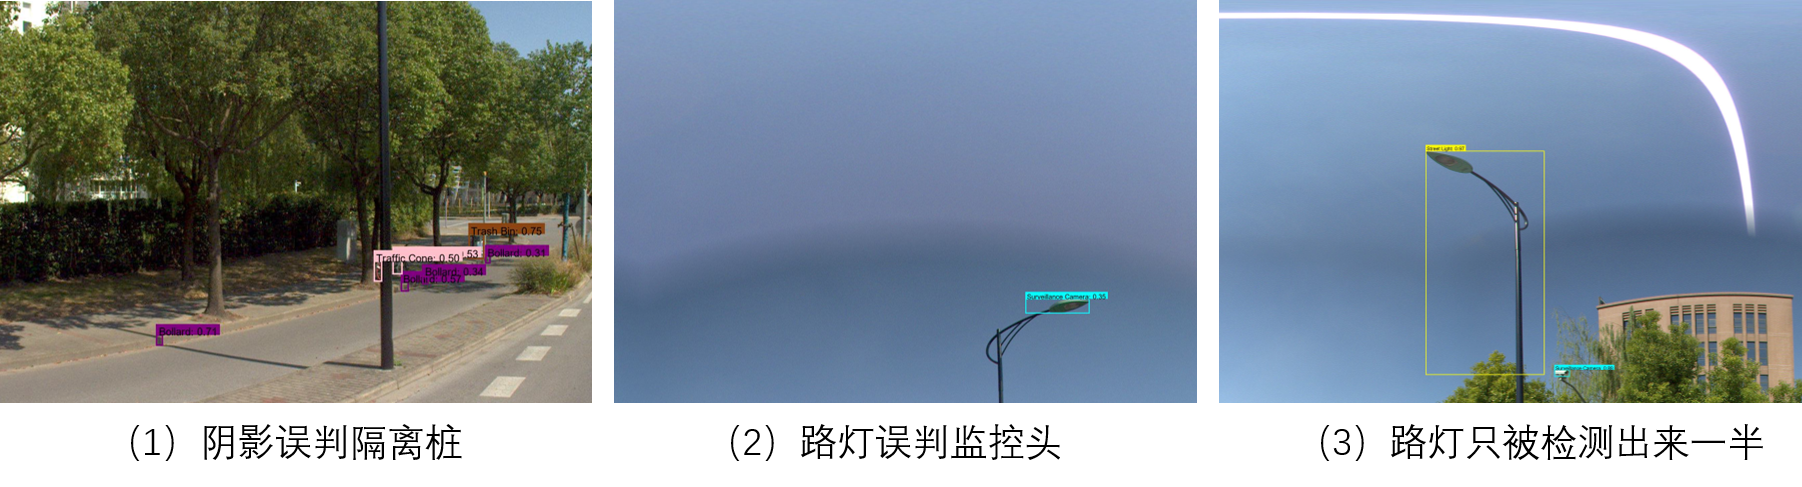
\includegraphics[width=1.0\textwidth]{logo/滑动窗口错误案例.png}
    \caption{固定滑窗切片检测引入无效区域与误检的典型案例}
    \label{fig:sliding_window_failure_cases}
\end{figure}

除量化指标外，主动感知三阶段检测相较于固定滑窗策略还有一项重要优势：其候选区域由第一阶段检测结果与场景语义先验共同约束，因此通常仅对具有复查价值的局部区域进行裁剪，而不会像规则滑窗那样引入大量缺乏有效前景的背景块。对于交通资产检测这类前景稀疏、背景占比高的任务，这一点尤为关键，因为阴影、天空、杆体边缘或建筑纹理等高对比背景都可能诱发新的误检。

图~\ref{fig:sliding_window_failure_cases} 给出了固定滑窗切片检测的三个典型失败案例。案例（1）中，规则窗口截取了路灯阴影等强纹理背景，模型将其误识别为隔离桩；案例（2）中，窗口包含大面积天空背景，而真实路灯仅有少量灯头被截入，导致上下文严重缺失，模型进一步误判为监控摄像头；案例（3）中，纵向尺度较大的长路灯仅有局部结构被截入窗口，目标整体几何形态被破坏，导致模型只能检测出目标物体的部分以致最终检测错误。需要指出的是，这类截断误差并不会因窗口重叠而自然消失：对于细长且跨越范围较大的目标，不同窗口往往只能覆盖其局部片段，难以提供完整结构线索，因此容易造成识别不完整、类别混淆或定位偏差。上述案例表明，固定滑窗虽然提高了局部覆盖率，但其裁剪结果缺乏任务相关性，容易因上下文不足或背景干扰而破坏检测判据。相比之下，本文方法通过 Crop Agent 主动选择高价值区域，在保留关键上下文的同时减少低信息量裁剪块进入第三阶段，从而降低无效推理与背景诱导误检的风险。

综合而言，固定步长重叠滑窗切片检测是一种强规则基线，其优势在于覆盖充分、实现直接，但代价是需要对 105 个局部窗口进行穷举检测，计算冗余显著，且无法区分高价值区域与低价值背景区域。相较之下，本文提出的主动感知三阶段检测并不依赖穷举遍历，而是利用全图初检结果与场景语义先验主动选择更值得复查的局部区域。实验结果表明，当 Crop Agent 与 Detection Agent 协同较好时，这种“先筛选、后精检”的策略能够以更低的局部检测预算获得更优或近似的检测性能；即便在与单阶段检测器的适配尚不充分时，也能保持接近规则滑窗的总体表现并取得更高的检测精度。因此，本文方法的关键优势不在于增加裁剪数量，而在于将局部检测由规则遍历转化为面向潜在漏检区域的主动搜索。

\subsubsection{Crop Agent 初始化方式对比}

除上述结构消融外，本文进一步比较 Crop Agent 的两种初始化方式：
\begin{itemize}
    \item \textbf{方案 A：}直接基于预训练 RexOmni 训练 Crop Agent；
    \item \textbf{方案 B：}基于已经在武汉数据集上微调收敛的 RexOmni，再训练 Crop Agent。
\end{itemize}

% 该实验用于分析：在进入 Crop Agent 训练之前，是否有必要先让基座模型完成交通资产场景适配。根据当前论文撰写进度，具体实验结果暂未填写，先在表~\ref{tab:crop_agent_init_compare} 中保留结果位置，以便后续补充。

\begin{table}[htbp]
    \centering
    \caption{不同 Crop Agent 初始化方式的对比结果}
    \label{tab:crop_agent_init_compare}
    \begin{tabular}{lcccc}
        \toprule
        初始化方式 & Macro-F1 & Micro-F1 & mIoU & Micro-IoU \\
        \midrule
        武汉微调 RexOmni $\rightarrow$ Crop Agent & 0.6328 & 0.6853 & 0.3828 & 0.4264 \\
        预训练 RexOmni $\rightarrow$ Crop Agent & -- & -- & -- & -- \\
        \bottomrule
    \end{tabular}
\end{table}

\subsection{方法局限性分析}

尽管本文方法在多数场景中均能够带来性能提升，但仍存在一定局限性。首先，当原始检测器对某些极端困难目标完全缺乏初始感知线索时，第二阶段候选区域推荐可能无法稳定捕获最优局部区域；其次，若局部区域内部背景极为复杂，或者目标本身存在严重遮挡与极端模糊，第三阶段局部精检的提升空间也会受到限制。

此外，在少数情况下，第三阶段局部检测可能引入与第一阶段部分重叠但并非完全重复的候选框，这说明候选区域选择与结果融合策略仍会对最终输出稳定性产生直接影响。后续工作可进一步结合区域置信度评估、自适应候选区域预算控制以及更细粒度的融合规则，对主动感知流程进行持续优化。

\section{本章小结}

本章围绕交通资产检测任务，系统介绍并验证了本文提出的基于主动感知的多智能体三阶段检测框架。方法上，本文完成了“全图初检—候选区域推荐—局部精检—结果融合”的整体流程设计，给出了 Crop Agent 训练数据构建方式、第三阶段局部精检机制以及跨阶段结果融合策略，从而将传统单次检测过程转化为面向潜在漏检区域的主动搜索过程。

实验结果表明，本文框架在多种 Detection Agent 上均具有良好的适配性和稳定增益，说明该方法具备较强的检测器无关性。进一步分析发现，本文方法的主要收益集中体现在小目标、密集区域和复杂局部场景中：通过候选区域推荐与局部精检，模型能够有效恢复原始全图检测遗漏的部分目标，并在 Precision、Recall、Macro-F1、Micro-F1 以及定位质量指标上获得不同程度提升。候选裁剪策略对比还表明，相比固定步长重叠滑窗，主动感知裁剪更能聚焦于高价值区域，能够减少纯背景裁剪、上下文截断和由无效区域引发的误检，因此具有更好的任务相关性与工程应用潜力。

此外，Crop Agent 初始化方式对比结果表明，直接基于预训练 RexOmni 训练 Crop Agent 的效果略优于基于领域微调模型继续训练的方案，说明候选区域推荐能力并不完全依赖于额外的场景适配。总体而言，本章从方法设计、整体性能、分尺度表现、裁剪策略有效性以及局限性分析等多个层面，验证了本文所提主动感知检测框架在交通资产检测任务中的有效性与实用价值。
